The activity diagrams show the basic flow of activities in the toll system. A customer can check in or out, or buy a toll tag, and a manager can get a report for a certain period. The enterprise manager can also change the price of toll tags and tickets.

\begin{figure}[H]
	\centering
	\begin{subfigure}[b]{0.3\textwidth}
	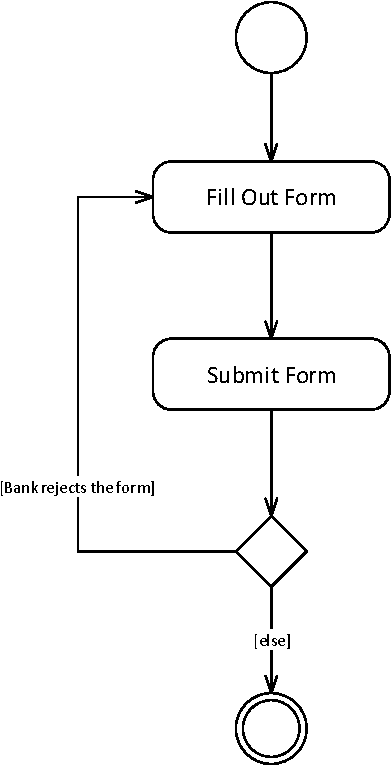
\includegraphics[width=\textwidth]{img/activity_diagram/buy_toll_tag}
	\caption{Activity diagram showing the process of buying a toll tag.}
	\end{subfigure}
	~
	\begin{subfigure}[b]{0.5\textwidth}
	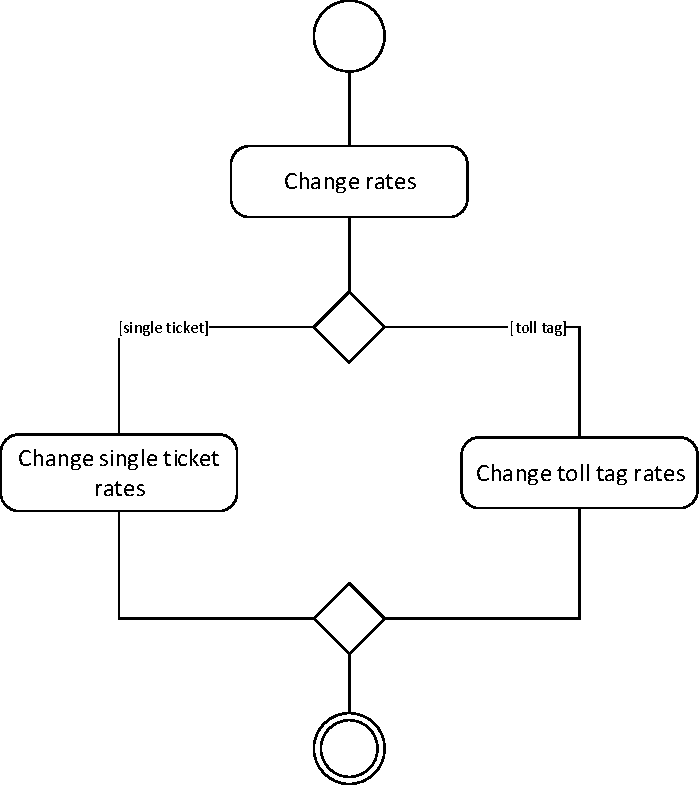
\includegraphics[width=\textwidth]{img/activity_diagram/change_rates}
	\caption{Activity diagram showing the process of changing the rate for toll tags or tickets.}
	\end{subfigure}
\end{figure}

\begin{figure}[H]
	\centering
	\begin{subfigure}[b]{0.6\textwidth}
	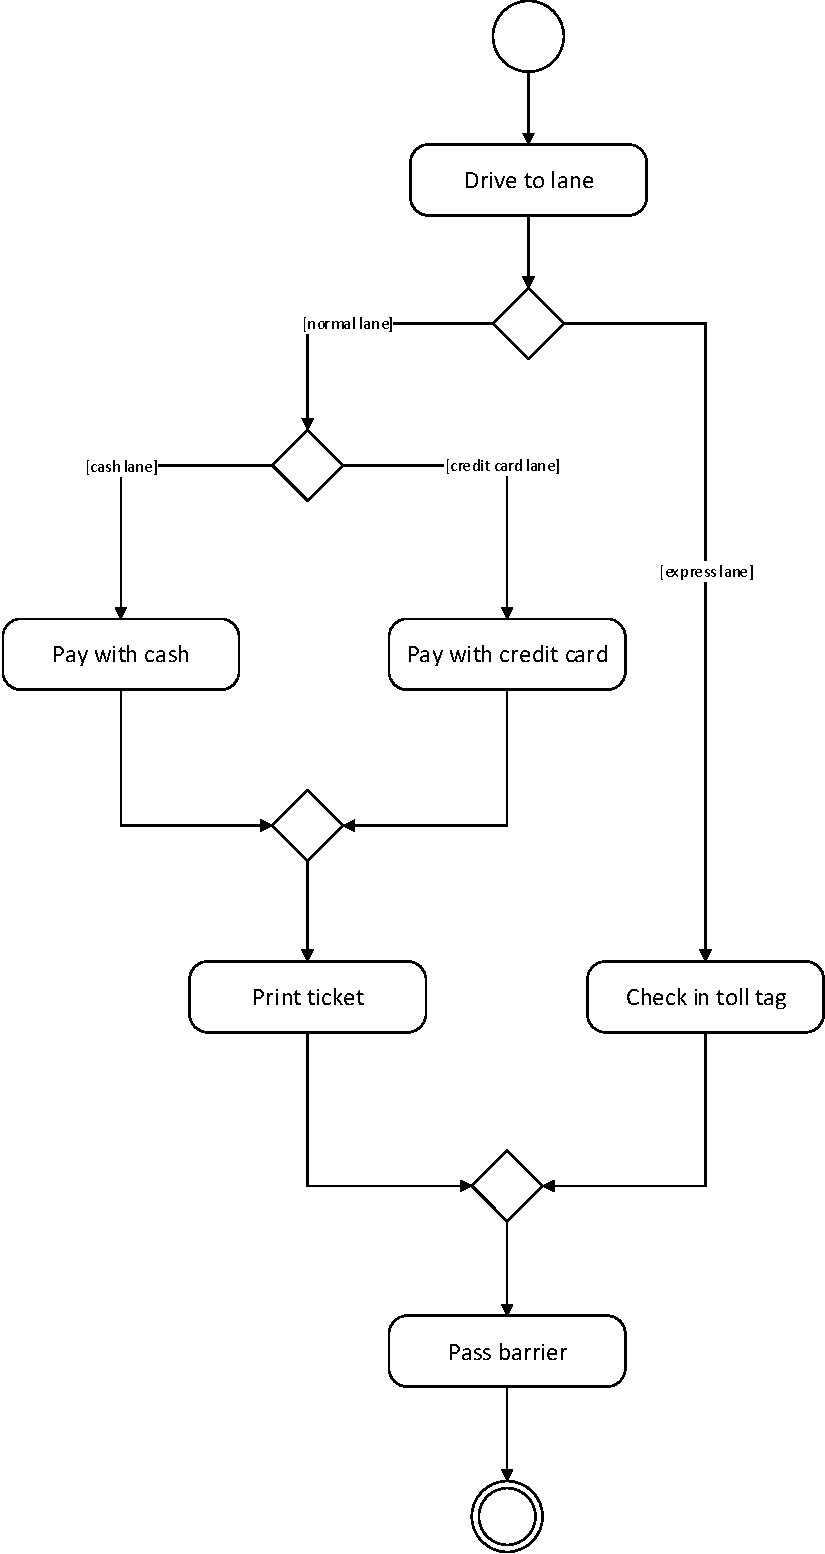
\includegraphics[width=\textwidth]{img/activity_diagram/check_in}
	\caption{Activity diagram showing how a customer checks in.}
	\end{subfigure}
\end{figure}

\begin{figure}[H]
	\centering
	\begin{subfigure}[b]{0.675\textwidth}
	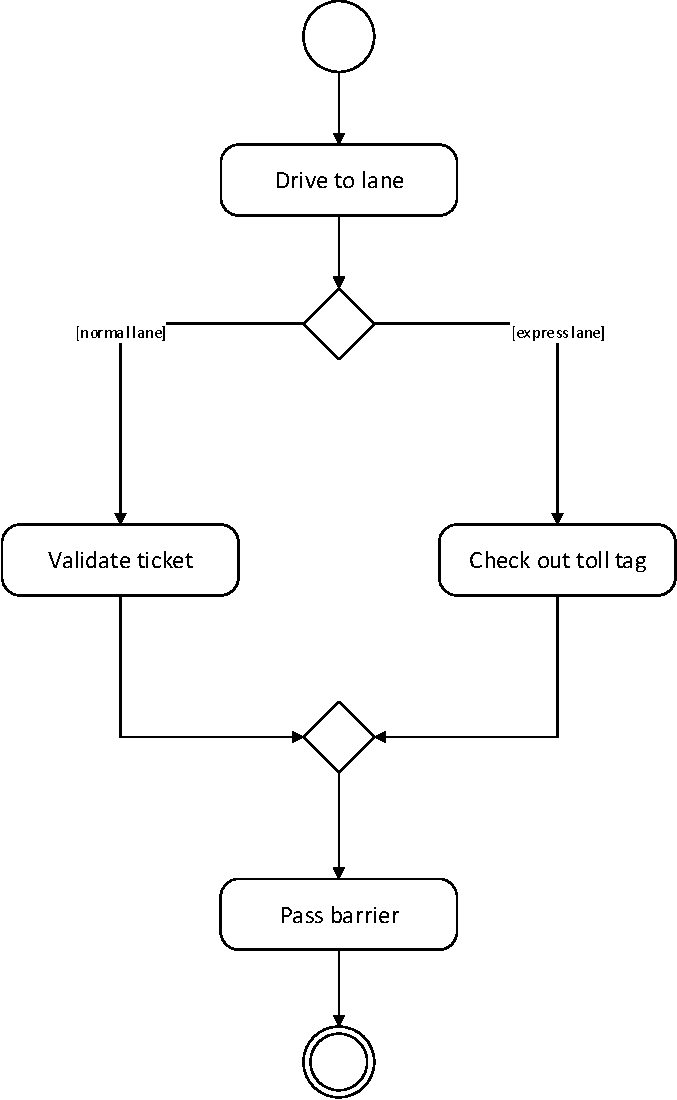
\includegraphics[width=\textwidth]{img/activity_diagram/check_out}
	\caption{Activity diagram showing how a customer checks out.}
	\end{subfigure}
	~
	\begin{subfigure}[b]{0.225\textwidth}
	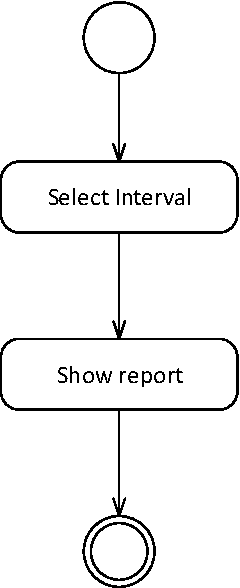
\includegraphics[width=\textwidth]{img/activity_diagram/show_report}
	\caption{Activity diagram showing how a manager gets a report.}
	\end{subfigure}
\end{figure}